Despite its many advantages, the NeXus file format is not particularly easy to work with for the uninitiated. This can be especially cumbersome to scientists who would much rather get their data and get on with their day. The NeXus Constructor is a tool written with \textit{Qt for Python} that attempts to address this problem by providing an interface for scientists to easily examine and modify the contents of NeXus files. \iffalse Such files can then be used for configuring the experiment control software in order to write real-time data. \fi The NeXus Constructor's interface consists of the following elements:

% Someone may not know what experiment control software does, what makes real-time data good, etc.

\begin{itemize}
\item Instrument View - A Qt3D pane that draws the experiment components in 3D. As NeXus files can contain information about a component's geometry and any transformations that may have been applied to it, translating this into something Qt3D can understand is fairly simple.
\item Component List - A list of the components in the NeXus file.
\item NeXus File Layout - An illustration of the hierarchical NeXus structure. Can't be used to see the values of the individual fields, but can serve as a tool through which you can check that the data has a sensible arrangement. Because the NeXus format is based on HDF5, the \texttt{h5py} library is able to interpret NeXus files so that we may display their layout in our application.
\end{itemize}

\begin{figure}
\caption{Screenshot of the NeXus Constructor}
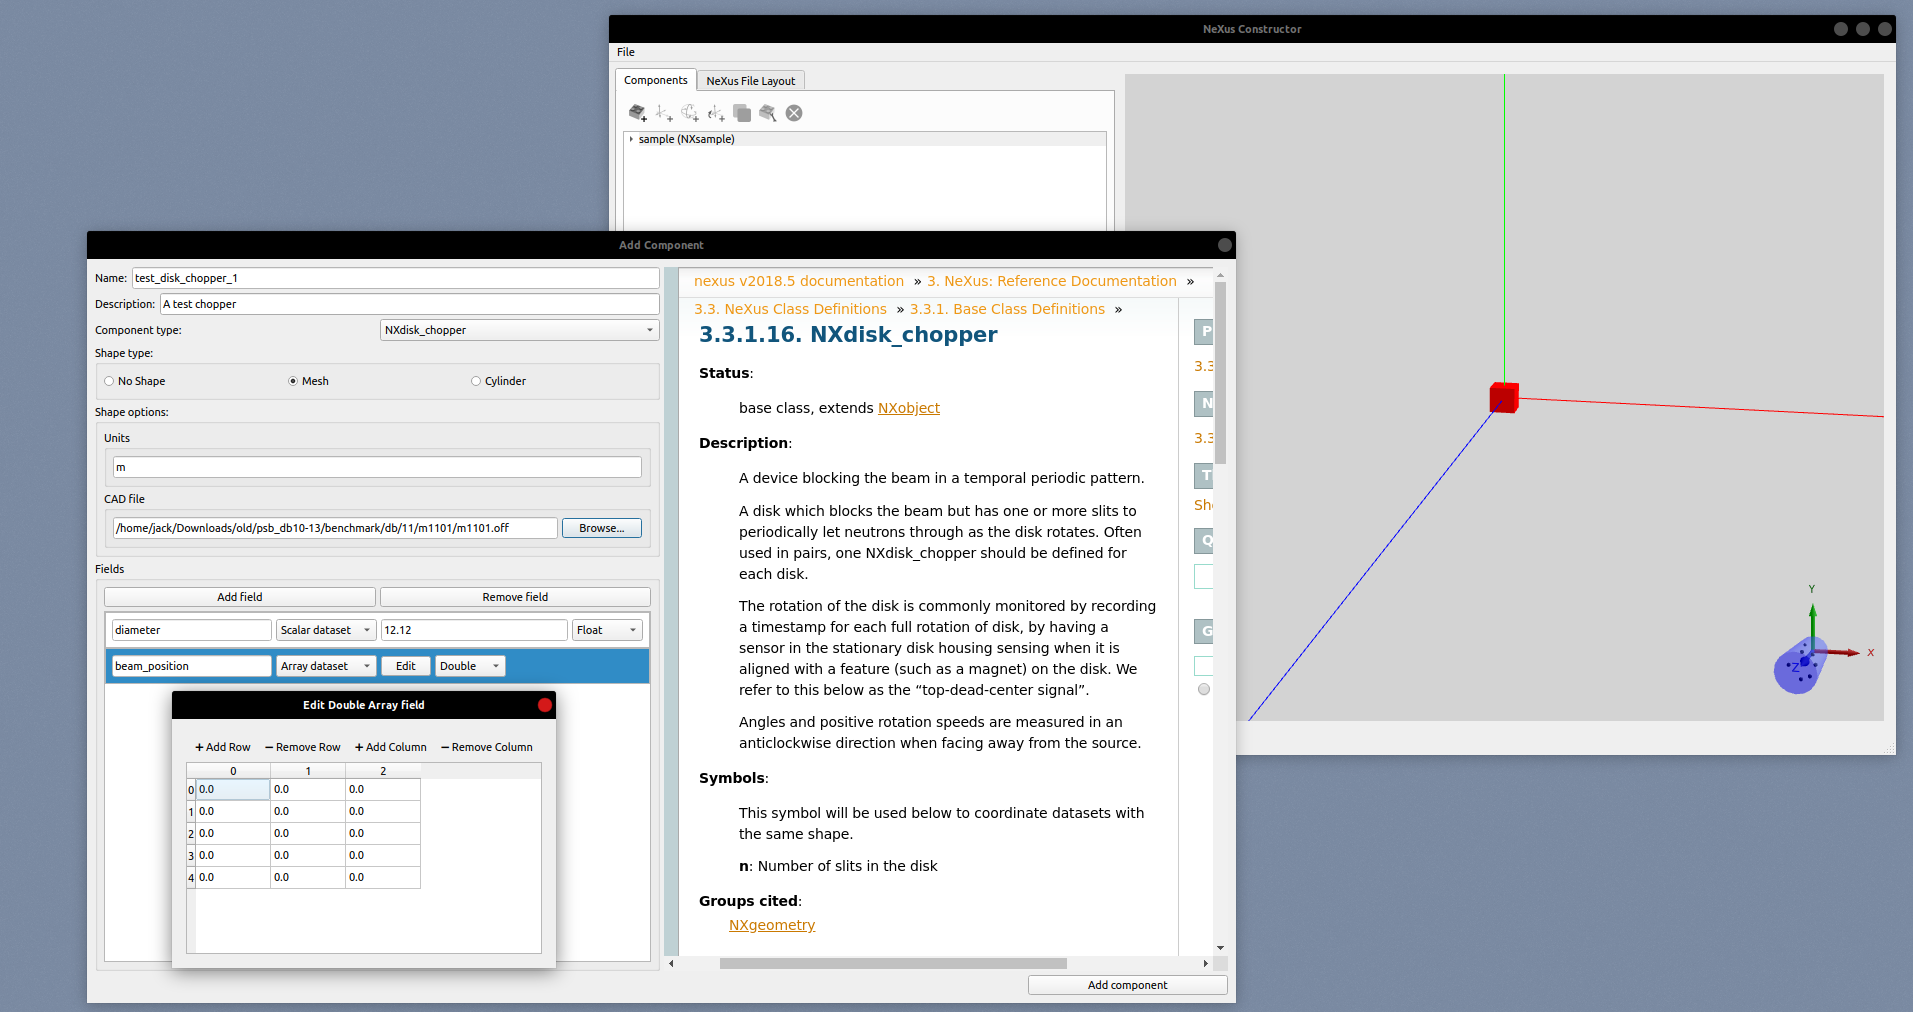
\includegraphics[width=\linewidth]{screenshot.png}
\end{figure}
